\chapter{Devices and technologies used}
\label{chapter:near-term}

After introducing the Ising model, our next task is to present the technologies used in the
research conducted for this thesis. Since the main point of this thesis is benchmarking quantum
annealers, it is only natural that we start by introducing the reader to the concepts of adiabatic
quantum computations and quantum annealing. The second part of the chapter is devoted to NVIDIA CUDA, a technology allowing massively parallel computations on general-purpose graphics processing
units (GPUs).


\section{Adiabatic quantum computation and quantum annealing}

\subsection{Adiabatic Quantum Computation}
One of the possible models of quantum computing is Adiabatic Quantum Computation (AQC)
\cite{farhi}. AQC ties closely with quantum annealing, and hence we will shortly discuss how it
works in general. Before we describe how the computations are performed in this model, we will take
a closer look at the underlying adiabatic theorem, which can be stated as follows \cite{farhi,
born}:

\begin{theorem}[Adiabatic theorem]
Suppose we are give a time-dependent Hamiltonian $\tilde{H}(t)$ with eigenenergies $E_1(t) \le E_2(t) \le
 \ldots \le E_i(t) \le \ldots$ and corresponding eigenstates $\ket{\psi_i(t)}$, Further, suppose we
 are given a physical system $\mathcal{S}$ evolving according to $H(t) = \tilde{H}(t/T)$ and let
 $\ket{\psi(t)}$ denote the state of $\mathcal{S}$ at time $t$. If $\ket{\psi(0)} =
 \ket{\psi_n(0)}$, then also $\ket{\psi(t)} = \ket{\psi_n(t)}$ for all time $t$, provided that $T$ is large
 enough and for all $t$ there
 exists a non-zero difference between $E_n(t)$ and the rest of the $H(t)$'s spectrum.
\end{theorem}

One conclusion to the adiabatic theorem is of particular importance to quantum computation. If the
system is prepared in a ground state, has a non-zero gap between its ground energy and the energy of
the first excited state, and is evolved slowly enough, it will stay in the ground state during the
whole evolution. Knowing we can finally discuss how AQC works. First, an optimization problem
to be solved is encoded as a ground state of some Hamiltonian $H_{target}$. Then, a physical system
is prepared in a ground state of some simpler hamiltonian, $H_{initial}$. After that, the system is
driven slowly from $H_{initial}$ to $H_{target}$. By adiabatic theorem, the system ends up in a
ground state of $H_{target}$, and after the measurement is performed the solution to the original
problem can be decoded.

In Quantum Annealing (QA), one follows essentially the same procedure as in Adiabatic Quantum
Computing. What is different, is that the evolution of the system in QA does not have to be
adiabatic \cite{Vinci2017}. Further, quantum annealing is not necessarily universal, with its
universality depending on the form of the Hamiltonians used and available ranges for the annealing
time. We will describe in more detail how Quantum Annealing works on a concrete example later in
this chapter when we discuss D-Wave annealers.

\subsection{D-Wave quantum annealers}

The first commercially available quantum annealer was D-Wave One, introduced by D-Wave company in
$2011$ \cite{johnson}. featuring 128 qubits. Since then, multiple improved generations of D-Wave
annealers have been released. At the time of writing, the newest series of D-Wave annealers is
called the Advantage system. Devices in this typically utilize a chip with at least
$5000$ qubits. Table \ref{tab:dwave} summarizes the release history of D-Wave annealers and
highlights the differences between their generations.

Number of qubits on chip is not the only factor restricting problems that can be submitted to the
annealer. To implement quadratic terms in the Ising hamiltonian, the qubits have to physically
interact. In all of the D-Wave devices manufactured so far, however, the connectivity is limited.
For instance, in devices from D-Wave 2000Q series, each qubit could interact with maximum of 6 other
qubits, whereas in Advantage systems qubit can havve up to 15 interacting neighbours. The
connectivity of qubits is determined by the device's \emph{topology}. We discuss topologies of
currently available D-Wave annealers, as well as the topology of the upcoming Advantage 2 system, in
deitals in the next section.

Topology describes an idealized graph, in which nodes correspond to the annealer's qubits and edges
map to couplers connecting them. In practice, however, some qubits or couplers might be unavailable
due to manufactiring errors or calibration problems. The actuall graph available on the device is
called its \emph{working graph}. Note that the working graph might change over time.

\begin{table}
    \footnotesize
    \label{tab:dwave}
\begin{tabular}[pos]{|l|c|c|c|c|}
\hline
\textbf{Series} & 
\textbf{Release year} &
\textbf{Topology} & 
\textbf{Num.\newline qubits} & 
\textbf{Num. couplers}\\ 
\hline    
D-Wave One & 2011 & Chimera $C_{4}$ & 128 & 352 \\
\hline
D-Wave Two & 2013 & Chimera $C_{8}$ & 512 & 1472 \\
\hline
D-Wave 2X & 2015 & Chimera $C_{12}$ & 1152 & 3360 \\
\hline
D-Wave 2000Q & 2017 & Chimera $C_{16}$ & 2048 & 6016\\
\hline
Advantage & 2020 & Pegasus $P_{16}$ & 5640 & 40484 \\
\hline
Advantage 2 & 2023-2024 & Zephyr $Z_{15}$ & 7440 & 71736 \\ 
\hline
\end{tabular}
\caption{Comparison of different generations of D-Wave annealers. The numbers of qubits and couplers
are given for a perfectly manufactured chip with full yield. Actual devices from any series
typically have a lower number of qubits and/or couplers.}.
\end{table}

\begin{figure}
    \centering
    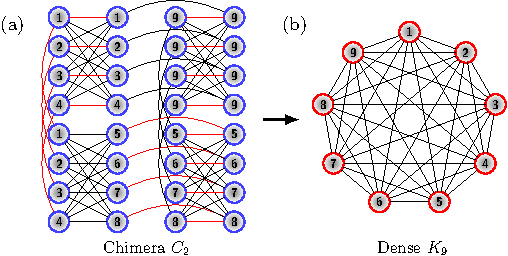
\includegraphics[width=\textwidth]{figures/chimera.pdf}
    \caption{\textbf{a.} Example of Chimera topology. Graph presented here consists of a $2 \times 2$ grid of unit cells (hence $C_2$ the name). Note the sparse connectivity of the presented graph as compared to the full graph with the same number of nodes. \textbf{b.} Full $K_9$ graph embedded in Chimera graph from \textbf{a.}. The nodes are labelled with numbers corresponding to groups of logical qubits they were constructed from.}
    \label{fig:chimera}
\end{figure}


\subsection{Annealer topologies}

The first D-Wave devices, up to Dwave 2000Q series (see Fig. \ref{fig:chimera}), used a to pology
called Chimera. 

The Ising model described in the previous chapter allows arbitrary interactions between spins. However, this is often not the case with physical devices like quantum annealers. For instance, in D-Wave devices, spins are arranged into a specific \emph{topology} with limited connectivity. Thus, the possible graph on which the optimization problems can be defined is much sparser than the complete $K_{N}$ graph. Spins in 2000Q devices are arranged in the so-called \emph{Chimera} topology depicted in figure \ref{fig:chimera}. The Chimera graph can be thought of as a $n \times m$ lattice of unit cells, where each cell is a complete bipartite $K_{4,4}$. Qubits are also connected to two qubits in neighbouring cells via external couplers (unless they reside on the border or a corner of the lattice), resulting in at most total 6 connections per qubit. Straightforward calculation shows that the Chimera graph has a total of $16mn + 4(m-1)n + 4(n-1)m$ edges.

The new Advantage system uses \emph{Pegasus} topology (see Fig \ref{fig:pegasus}), which increases
the maximum degree of vertex in the graph to 15. For the details of this topology, we refer the interested
reader to \cite{boothby}.
\todo[inline]{instead of only citing, describe pegasus}


\begin{figure}
    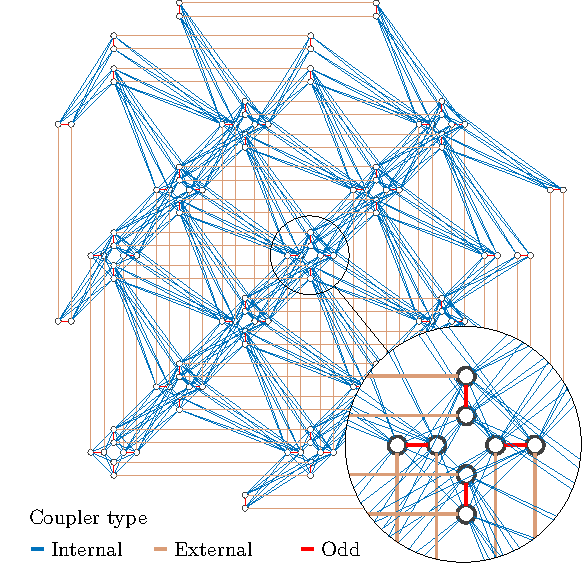
\includegraphics[width=\textwidth]{figures/pegasus}
    \caption{
        The $P_3$ graph, an example of the Pegasus topology. Different types of couplers are
        color--coded. The magnified portion of the image shows a part of the graph containing a
        Chimera unit cell. Observe the inner couplers, marked in red, connecting qubits that are not
        connected in Chimera topology. The addition of these couplers allows for running problems
        that are not necessarily defined on a bipartite graph.
    }
\end{figure}
\subsection{Minor embeddings}

Not every Ising problem one might wish to solve is compatible with the topology of physical quantum annealer. This issue can sometimes be circumvented using a procedure called \emph{minor embedding}. In this approach, one considers groups of several physical spins connected in a chain as a single logical one. Vertices corresponding to spins in each such chain are contracted, resulting in the new graph, having higher connectivity but smaller number of vertices than the original one. With the proper choice of chains, this new graph can contain a subgraph isomorphic to the graph of the problem to solve. The minor embedding process is illustrated in figure \ref{fig:chimera}.

Grouping qubits into chains and contracting them is not enough to run the embedded problem. One first has to ensure that all spins in a chain align in the same direction, so that they can indeed represent a single logical variable. This is accomplished by adding a penalty term which prohibitively increases the cost of solutions in which the value of spins in chains differ. However, due to the probabilistic nature of quantum annealer, even after adding penalty one might obtain solutions in which values of spins in some chains disagree. Such disagreeing chains are called \emph{broken}. Since solutions containing broken chains cannot be interpreted directly as a solution to the original problem, one has to either discard them, or manually correct them (e.g. by choosing the most common value among the spins in the chain).

% To define minor embedding more formally, let us first define the notion of vertex contraction. Let $(G, E)$ be a graph defining topology of the device and let $v_{1}, \ldots, v_{{n}} \in E$ be a chain of vertices. Contraction of vertices $v_{1}, \ldots, v_{n}$ is a new graph $G'=(V', E')$ such that
% \begin{itemize}
%   \item $V' = V \setminus \{v_{1}, \ldots, v_{{n}}\} \cup \{w\}$, where $w$ is some new vertex.
%   \item $E' = \{e \in E\colon v_{i} \notin E\} \cup \{\{v, w\}\colon \exists_{i} \{v, v_{i}\} \in E\}$
% \end{itemize}
% Intuitively, contracting vertices replaces them with a new one connected with their every neighbour.

\subsection{Comparison to classical model of computation}
It is clearly visible that quantum annealing is different from computing using classical computers. One of the most obvious differences is computational model. On classical computers, one essentially writes programs as a series of instructions to be executed by the CPU. On typical machines, CPU is capable of performing arithmetic operations, computing values of some special functions, managing execution flow, controlling I/O and much more. In comparison, quantum annealers are capable of executing a single operation: annealing given optimization problem. Therefore, programming these devices boils down to defining an optimization problem and tuning the annealing parameters. There is no processing flow controlled by the programmer.

Another difference between classical computers and quantum annealers is lack of working memory in the former. Classical computers use working memory (typically in the form of RAM) to store machine code and data. However, quantum annealers do not need to store neither code nor data, and hence they do not feature an analogous component. Similarly, quantum annealers, being purely computational oriented devices, do not have mass storage.

A slightly less obvious difference between classical computers and quantum annealers is their model of parallelism. Classical computers are capable of running several threads of execution at the same time. However, every non-trivial classical algorithm involving parallelism must necessarily also include a serial part, which limits speed-up gained for introducing more CPU cores or CPUs. In contrast, quantum annealers are capable of annealing multiple qubits at the same time, which makes their operation inherently parallel.

\section{Nvidia CUDA}

Quantum annealing, introduced in the previous section, is an inherently heuristic process. Like many heuristic algorithms, it cannot certify that the solution it found is in fact optimal. One way to assess performance of such algorithms is to compare their results with known low-energy spectrum of some test instances. In this section, we describe the Nvidia CUDA technology, which we use for our implementation of massively parallel brute-force algorithm describe in chapter \ref{chapter:bruteforce}.

\subsection{Brief history of Graphics Processing Units}
The history of specialized hardware for manipulating graphics ranges as far as the 1970s. Initially these devices, that later became known as Graphics Processing Units (GPU), offered limited functionalities. Increasing demand for performance in gaming industry and professional graphics processing drove the evolution of GPUs, which quickly became highly sophisticated devices supporting advanced 2D and 3D image manipulation. Performing such arithmetically intensive operations requires enormous computational power, and it was only the matter of time until it was realised that the power of these devices can be harnessed for general purpose computations (so called GPGPU - General Purpose computing on GPU).

Early efforts in development of GPGPU required framing of computational problem in terms of operations performed on graphical primitives, as this was the only way for using specialized API of GPUs. This changed with the development of devices and toolkits that supported operations needed for general purpose computations out of the box. Notably, in 2007 Nvidia introduced its massively parallel CUDA architecture.

\subsection{Differences between CPU and GPU}
Principles behind operation of CUDA-enabled devices are fundamentally different from the ones governing execution of program on traditional CPU-only architecture. In current x86 based computers, the CPU runs a given sequence of instructions (so-called thread of execution) using one of its cores. Such a processor is the ''brain'' of a computer, and it can perform a wide variety of tasks ranging from arithmetic operations, through accessing the system's RAM, to performing IO operations and controlling other components of the system. Typical CPUs are optimized for sequential execution, and as such are usually equipped with moderate (as compared to the GPUs) number of high-performance cores.

On the other hand, GPUs are more specialized. They are well suited for performing numerous arithmetic operations and accessing memory in parallel. They typically have more cores than a traditional CPU (with even modern commodity GPUs boasting thousands of them). Although those cores are less performant than their CPU counterparts and support a much narrower set of operations, their large number combined with fast memory access gives modern GPUs advantage over CPUs in multiple areas.

\subsection{Processing flow on CUDA}
Considering the architectural differences between CPUs and GPUs, it is hardly surprising that both of these types of devices are programmed quite differently. The first major difference is that GPUs cannot operate on their own and are themselves controlled by CPU. This is why CUDA is a type of \emph{heterogenous} architectures (as opposed to CPU-only \emph{homogenous} architectures). The processing flow on CUDA is summarized in Figure \ref{fig:cuda_flow}.

\begin{figure}[ht]
    \centering
    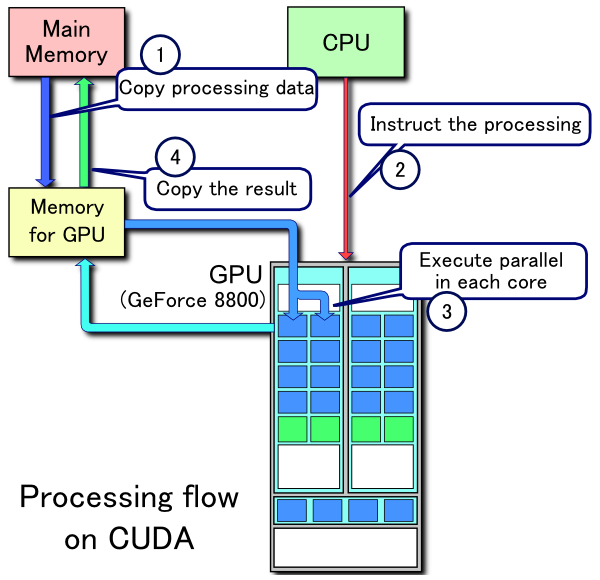
\includegraphics[width=0.7\textwidth]{figures/CUDA_processing_flow_(En).png}
    \caption{{\protect\todo[inline]{Important: this figure is only here temporarily, I will prepare my own graph once the text is done.}} Processing flow on CUDA. The CPU sends input data to the GPU memory, and launches the computational kernel. The kernel's code is executed, in parallel, using multiple threads on GPU. Once the execution is done, results are copied from the GPU memory to the system's RAM.}
    \label{fig:cuda_flow}
\end{figure}

Programs run on GPU are organized in \emph{kernels}. For the most part, kernels might be viewed as functions or subroutines (which is indeed how they are implemented) that don't have a return value. On a CPU, such function would be executed by some core as a part of a thread. In CUDA however, the very same kernel is executed by multiple threads. Executing a kernel requires specifying a \emph{grid} that will be used for running it. A grid can be 1, 2- or 3-dimensional and is itself divided into blocks. Each block is in turn also organized in 1, 2, or 3-dimensional structure of threads (the same for every block in the grid). A schematic view of a two-dimensional grid is presented on Figure \ref{fig:cuda_grid}.

\begin{figure}[ht]
    \centering
    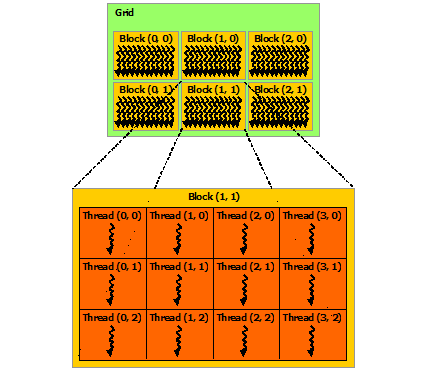
\includegraphics[width=0.8\textwidth]{figures/grid-of-thread-blocks.png}
    \caption{{\protect \todo[inline]{This is also a temporary figure...}} A schematic view of an example two-dimensional CUDA grid. Presented here is a 2 $\times$ 3 grid of 3 $\times$ 4 blocks.}
    \label{fig:cuda_grid}
\end{figure}

As already mentioned, each thread in the grid executes \emph{precisely the same} kernel. It might therefore seem surprising that, nevertheless, they are able to access different parts of memory. This is possible, because each thread is identified by its indices in both the grid and the block. Those indices can be used e.g. for computing offsets in arrays that are being processed. A more sophisticated use of thread and block indices will be exemplified in chapter \ref{chapter:bruteforce}.

\subsection{SIMT architecture}
CUDA-enabled GPUs employ an architecture called SIMT (Single Instruction, Multiple Threads)\footnote{One can contrast SIMT architecture used by CUDA with SIMD instructions (Single Instruction, Multiple  Data) available on mother CPUs.}. As implied by the name, in SIMT architecture, multiple threads execute the same instruction. Threads are executed in blocks  by computational units called Streaming Multiprocessors (SMs), and blocks distributed to multiprocessors on kernel launch. When a block is distributed to SM, it is further partitioned into \emph{warps}, groups of 32 threads each. All threads in a warp are scheduled for execution together. Nevertheless, they have separate program counter and thus their execution flow can diverge. At any given time, a  thread in a warp can be either active (executing \emph{the same} instruction as the rest of the active threads in a warp) or inactive (not executing any instruction at all). A thread may be inactive because its execution diverged from the rest of the warp or because it terminated earlier. It is interesting to note that starting from the Volta architecture, threads can be scheduled on finer level of granularity, allowing them to diverge and reconverge on the sub-warp level. Each multiprocessor manages a set of 32-bit registers and parallel data cache, called \emph{shared memory}, distributed among the thread blocks. Since those resources are limited, the number of warps that can run in parallel on any SM is heavily dependent on resource usage of the kernel being executed.

\subsection{Memory hierarchy}

Threads can access several memory types during kernel execution, including global memory, local memory, constant and texture memory and shared memory. Physically, those different memory types can be divided into device memory (global memory, local memory, constant memory) and on-chip memory (shared memory). SM's on-chip memory also serves as L1 cache.

Global memory is a device memory available to each thread. All accesses to global memory are serviced in 32-, 64-, or 128- bytes memory transactions. Accesses made from a single warp are coalesced into as many of such transactions as necessary, depending on devices compute capability and access pattern. Reads and writes targeting global memory are always cached in L2 and (depending on configuration, compute capability and access pattern) may also be cached in L1 cache.

Local memory resides physically on the device, and thus offers the same bandwidth and latency. Just like global memory, it is always cached in L2 cache. This type of memory is never used directly by the programmer. Instead, the compiler might decide to use it for local variables of a thread in case there is not enough register (so-called \emph{register spilling}) or for dynamically indexed local arrays. Local memory is arranged in such a way, that accesses are always fully coalesced as long as all threads access the same relative address (e.g. the same local variable, the same index of local array etc.).

Constant memory and texture memory are two types of read-only memory \footnote{Read-only here means ``Not writeable from inside the kernel''} residing in global memory. Accesses to constant memory are cached in constant cache and accesses to it are serialized. Therefore, each request is split into as many  transactions as there are different memory addresses in the original request. Texture memory is cached in texture cache, which is optimized for accessing spatial data. Hence, the best performance is achieved if threads in a warp read or write to the addresses that are close in 2D.

Threads can cooperate and share data through the use of on-chip \emph{shared  memory}. The amount of allocated shared memory is directly controlled by the programmer either on the kernel definition level, or during its launch. Shared memory is organized in banks that can be accessed simultaneously, and the best performance is achieved if each thread in a warp accesses memory in a different bank. Otherwise, a \emph{bank conflict occurs}, and the request is split into as little conflict-free requests as possible.


\subsection{Programming environment}
CUDA devices can be programmed directly using either C/C++ or Fortran. The C/C++ code can be compiled using Nvidia's nvcc compiler, shipped out of the box with CUDA toolkit, while using Fortran requires installing its third-party distribution (e.g. PG Fortran developed by Portland Group). Giving a comprehensive walkthrough of using either C/C++ or Fortran with CUDA is well beyond the scope of this thesis, but for the sake of completeness we present a short example of CUDA Fortran code in listing \ref{lst:cuda_fortran} \todo{Note to self: remember to either replace it with my own example or cite the source (CUDA Fortran documentatoin)}.

\begin{lstlisting}[
    language=Fortran,
    label=lst:cuda_fortran,
    captionpos=b,
    caption={Example code in CUDA Fortran. Presented here are an example kernel performing saxpy operation together with a host subroutine that uses it.},
    frame=tlrb,
    aboveskip=2em,
    belowskip=2em
]{fortran}
! Kernel definition
attributes(global) subroutine ksaxpy( n, a, x, y )
   real, dimension(*) :: x,y
   real, value :: a
   integer, value :: n, i
   i = (blockidx%x-1) * blockdim%x + threadidx%x
   if( i <= n ) y(i) = a * x(i) + y(i)
end subroutine

! Host subroutine
subroutine solve( n, a, x, y )
   real, device, dimension(*) :: x, y
   real :: a
   integer :: n
   ! call the kernel
   call ksaxpy<<<n/64, 64>>>( n, a, x, y )
end subroutine
\end{lstlisting}

Along to the nvcc compiler, the CUDA toolkit contains several, more specialized libraries. Among others, those include:
\begin{itemize}
    \item cuBLAS -- CUDA Basic Linear Algebra Subroutines library,
    \item cuFFT -- CUDA Fast Fourier Transform library,
    \item cuRAND -- CUDA Random Number Generation library,
    \item cuSPARSE -- CUDA library for manipulating sparse matrices.
\end{itemize}
For many high-level languages, there exist third-party wrappers enabling use of CUDA (e.g. PyCuda for Python).



%%% Local Variables:
%%% mode: latex
%%% TeX-master: "../main"
%%% End:
